\section{Pivotal configurations.}
Fix a dipolar tree $T$.
Let us label the poles of $T$ by $p_1$ and $p_2$ and the reaming vertexes by $x_1,x_2,\dots,x_n$.

Assume $A$ is a complete $\CBB[0]$ length space.

A point array $p_1,p_2,x_1,\dots x_n\in A$ together with choice of one geodesic connecting adjacent vertexes of $T$ will be called \emph{geodesic $T$-tree};
it contains one geodesic $[p_1,p_2]$ and $n$ geodesics  $[p_i,x_j]$.
A geodesic tree be denoted as 
$[p_1,x_1\dots x_k(p_2,x_{k+1}\dots x_n)]$;
meaning that $p_1$ connected to $x_1,\dots,x_k$ and $p_2$ and $p_2$ is connected to $x_{k+1},\dots x_n$

A geodesic tree  $\~T=[\~p_1,\~x_1\dots \~x_k(\~p_2,\~x_{k+1}\dots \~x_n)]$ in $\HH$ will be called \emph{pivotal tree} for $T=[p_1,x_1\dots x_k(p_2,x_{k+1}\dots x_n)]$
if 
\begin{enumerate}[(i)]
\item $|\~p_1-\~p_2|= |p_1-p_2|$,
\item $|\~p_i-\~x_j|= |p_i-p_j|$ for any edge $[p_i,x_j]$ in $T$ and
\item $\measuredangle[\~p_j\,^{\~x_k}_{\~p_i}]_{\HH}=\measuredangle[\~p_j\,^{\~x_k}_{\~p_i}]_A$
for any hinge  $[p_j\,^{x_k}_{\~p_i}]$ in $T$.
\end{enumerate}

\begin{thm}{Rigidity lemma}\label{lem:rigidity}
Let $A$ be a complete $\CBB[0]$ length space.
Suppose  $[\~p_1,\~x_1\dots \~x_k(\~p_2,\~x_{k+1}\dots \~x_n)]$ is a pivotal tree for a geodesic tree  with the vertexes $[p_1,x_1\dots x_k(p_2,x_{k+1}\dots x_n)]$ in $A$.
Assume that
\[|\~x_i-\~x_j|_\HH\le |x_i-x_j|_A 
\eqlbl{eq:pivotal-comparison}\]
for any pair $(i,j)$ and the convex hull $\~K$ of $\{\~x_1,\dots\~x_n\}$ intersects the line $\~p_1\~p_2$.
Then in \ref{eq:pivotal-comparison} we have equality for each pair $(i,j)$.
\end{thm}

\parit{Proof.}
Assume that a point $\~z$ on the line $(\~p_1,\~p_2)$ is given.
We can assume that $\~z$ lies on the half-line $[\~p_1,\~p_2)$;
otherwise swap  $\~p_1$ and $\~p_2$.

Denote by $\zeta$ the direction of geodesic $[p_1,p_2]$ at $p_1$. 
Set $z=\gexp_p(|\~z-\~p_1|\cdot \zeta)$, where $\gexp$ denotes the gradient exponent; see \cite{AKP-book}. 
By comparison, we have
\begin{align*}
|x_i-z|_A &\le |\~x_i-\~z|_{\RR^2}
\end{align*}
for any $i$.

It remains to apply Kirszbraun rigidity theorem (\ref{thm:kirszbraun-rigid}).
\qeds

Suppose  $[\~p_1,\~x_1\dots \~x_k(\~p_2,\~x_{k+1}\dots \~x_n)]$ is a pivotal tree for a geodesic tree  with the vertexes $[p_1,x_1\dots x_k(p_2,x_{k+1}\dots x_n)]$ in $A$.
Note that by angle comparison 
\[|\~x_i-\~p_j|_{\RR^n}\ge |x_i-p_j|_A\]
for any $i$ and $j$.
It follows that the configuration $\~p_1$, $\~p_2$, $\~x_1,\dots\~x_n\in \HH$ satisfies the tree comparison (see Section~\ref{sec:intro}) if 
\[|\~x_i-\~x_j|_{\RR^n}\ge |x_i-x_j|_A
\eqlbl{eq:tree-comparison}\]
for all pairs $(i,j)$.

Denote by $\xi_i$ the direction of the half-plane thru $\~x_i$ with the boundary line $(\~p_1, \~p_2)$.
We may assume that all $\xi_i$ belong to a unit sphere, of dimension at most $n-1$.
Note that up to a motion of $\HH^n$, a pivotal configuration is completely described by the angles $\measuredangle(\xi_i,\xi_j)$.

Let us denote by $\alpha_{i,j}$ the minimal angle $\measuredangle(\xi_i,\xi_j)$ in a pivotal configuration such that $|\~x_i-\~x_j|_{\RR^3}\ge|\~x_i-\~x_j|_A$. 
Note that the enequality \ref{eq:tree-comparison} holds if and only if 
\[\measuredangle(\xi_i,\xi_j)\ge \alpha_{i,j}.\]

\begin{thm}{Corollary}\label{cor:|x-x|}
For any geodesic dipolar tree  in a complete $\CBB[0]$ length space the following conditions hold:
\begin{enumerate}[(a)]
\item For any pair $i$ and $j$, we have
\[\alpha_{i,j}\le \pi.\]
\item For any triple $i$, $j$ and $k$,  we have
\[\alpha_{i,j}+\alpha_{j,k}+\alpha_{k,i}\le 2\cdot\pi.\]
\end{enumerate}
In other words, if $A$ is a nonnegatively curved complete length space then
\begin{enumerate}[(a)]
\item\label{cor:|x-x|:a} For any broken geodesic line $[p_1,x_1(p_2,x_2)]$ in  $A$ there is a pivotal tree $[\~p_1,\~x_1(\~p_2,\~x_2)]$ such that 
\[|\~x_1-\~x_2|_{\HH}\ge |x_1-x_2|_A.\]

\item\label{cor:|x-x|:b} For any geodesic tree $[p_1,x_1x_2(p_2,x_3)]$ in $A$ there is a pivotal tree $[\~p_1,\~x_1\~x_2(\~p_2,\~x_3)]$ such that 
\begin{align*}
|\~x_1-\~x_2|_{\HH}&\ge |x_1-x_2|_A,
\\
|\~x_2-\~x_3|_{\HH}&\ge |x_2-x_3|_A,
\\
|\~x_3-\~x_1|_{\HH}&\ge |x_3-x_1|_A.
\end{align*}
\end{enumerate}

\end{thm}
\begin{comment}
\begin{wrapfigure}{r}{15 mm}
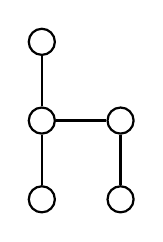
\begin{tikzpicture}[scale=1,
  thick,main node/.style={circle,draw,font=\sffamily\bfseries,minimum size=3mm}]
  \node[main node] (1) at (0,0) {};
  \node[main node] (2) at (0,1){};
  \node[main node] (3) at (0,2){};
  \node[main node] (4) at (1,0) {};
  \node[main node] (5) at (1,1) {};
  

  \path[every node/.style={font=\sffamily\small}]
   (1) edge node[above]{}(2)
   (2) edge node[above]{}(3)
   (2) edge node[above]{}(5)
   (4) edge node[above]{}(5);
\end{tikzpicture}
\end{wrapfigure}
\end{comment}

Note that the part \textit{(\ref{cor:|x-x|:b})} implies that $A$ satisfies tree comparison for the tree as on the digram. 
In the next section we will use it to prove stronger statements.

The part \textit{(\ref{cor:|x-x|:a})} can be also interpreted as a tree comparison for the three isomorphic to the path with three edges;
however, this comparison holds in any metric space --- it follows directly from the triangle inequality.

\section{Six point comparison}


\begin{thm}{Theorem}
Let $A$ be an complete nonnegatively curved lenght space.
Then for any tree $[p_1,x_1x_2x_3(p_2,x_4)]$ and $[p_1,x_1x_2(p_2,x_3x_4)]$ (see the diagram) there is a pivotal tree satisfying the tree comparison.

In particular, any complete nonnegatively curved lenght space satisfies the comparison for 
 2(2) and 3(1) bipolar trees.

\begin{comment}
\begin{center}
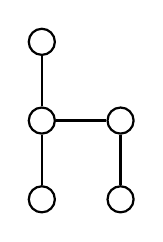
\begin{tikzpicture}[scale=1,
  thick,main node/.style={circle,draw,font=\sffamily\bfseries,minimum size=3mm}]
  \node[main node] (1) at (0,0) {};
  \node[main node] (2) at (0,1){};
  \node[main node] (3) at (0,2){};
  \node[main node] (4) at (1,0) {};
  \node[main node] (5) at (1,1) {};
  

  \path[every node/.style={font=\sffamily\small}]
   (1) edge node[above]{}(2)
   (2) edge node[above]{}(3)
   (2) edge node[above]{}(5)
   (4) edge node[above]{}(5);
\end{tikzpicture}
\hskip10mm
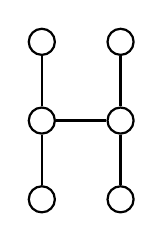
\begin{tikzpicture}[scale=1,
  thick,main node/.style={circle,draw,font=\sffamily\bfseries,minimum size=3mm}]

  \node[main node] (1) at (0,0) {};
  \node[main node] (2) at (0,1){};
  \node[main node] (3) at (0,2){};
  \node[main node] (4) at (1,0) {};
  \node[main node] (5) at (1,1) {};
  \node[main node] (6) at (1,2) {};

  \path[every node/.style={font=\sffamily\small}]
   (1) edge node[above]{}(2)
   (2) edge node[above]{}(3)
   (2) edge node[above]{}(5)
   (4) edge node[above]{}(5)
   (5) edge node[above]{}(6);
\end{tikzpicture}
\hskip10mm
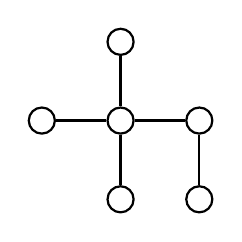
\begin{tikzpicture}[scale=1,
  thick,main node/.style={circle,draw,font=\sffamily\bfseries,minimum size=3mm}]

  \node[main node] (1) at (0,1) {};
  \node[main node] (2) at (1,0){};
  \node[main node] (3) at (1,1){};
  \node[main node] (4) at (1,2) {};
  \node[main node] (5) at (2,0) {};
  \node[main node] (6) at (2,1) {};

  \path[every node/.style={font=\sffamily\small}]
   (1) edge node[above]{}(3)
   (2) edge node[above]{}(3)
   (3) edge node[above]{}(6)
   (4) edge node[above]{}(3)
   (5) edge node[above]{}(6);
\end{tikzpicture}
\end{center}
\end{comment}

\end{thm}


\parit{Proof.} 
Let us fix a geodesic tree $[p_1,x_1x_2x_3(p_2,x_4)]$ and $[p_1,x_1x_2(p_2,x_3x_4)]$.
The rest of the proof in these two cases will be identical.
Recall that $p_1$ and $p_2$ are the poles of the tree and each of remaining vertexes $\xi_1,\xi_2, \xi_3,\xi_4$ are connected to one of the poles.

Define the values $\{\alpha_{i,j}\}$ for each pair $i,j$ as in the previous section.
The following algorithm, produces a metric graph with the vertexes denoted by $\xi_1,\xi_2, \xi_3,\xi_4$.
\begin{enumerate}[1.]
\item List the values $\{\alpha_{i,j}\}$ in the non-increasing order.
\item If $\alpha_{i,j}$ the first value in the list, connect vertexes $\xi_i$ and $\xi_j$ by an edge of length $\alpha_{i,j}$.
\item Do the same for the second value  in the list.
\item Starting from the third step, we attach a new edge corresponding to the next value $\alpha_{i,j}$ only if the already constructed edges in the graph will remain to be the shortest path between their vertexes; otherwise go to the next value in the list. 
\item Repeat until the end of the list.
\end{enumerate}
Denote the obtained metric graph by $\Gamma$;
note that $\Gamma$ is connected. 

If the triangle inequalities 
\[\alpha_{i,k}\le \alpha_{i,j}+\alpha_{j,k}\]
hold for all triples $(i,j,k)$, then $\Gamma$ is the complete graph with 4 vertexes;
otherwise it will be one of the following graphs.

\begin{comment}
\begin{center}
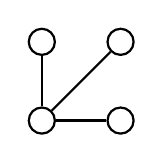
\begin{tikzpicture}[scale=1,
  thick,main node/.style={circle,draw,font=\sffamily\bfseries,minimum size=3mm}]

  \node[main node] (1) at (0,0) {};
  \node[main node] (2) at (0,1){};
  \node[main node] (3) at (1,1){};
  \node[main node] (4) at (1,0) {};

  \path[every node/.style={font=\sffamily\small}]
   (1) edge node[above]{}(2)
   (1) edge node[above]{}(3)
   (1) edge node[above]{}(4);
   
\end{tikzpicture}
\hskip10mm
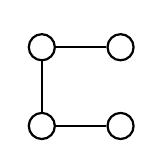
\begin{tikzpicture}[scale=1,
  thick,main node/.style={circle,draw,font=\sffamily\bfseries,minimum size=3mm}]

  \node[main node] (1) at (0,0) {};
  \node[main node] (2) at (0,1){};
  \node[main node] (3) at (1,1){};
  \node[main node] (4) at (1,0) {};

  \path[every node/.style={font=\sffamily\small}]
   (1) edge node[above]{}(2)
   (2) edge node[above]{}(3)
   (1) edge node[above]{}(4);
\end{tikzpicture}
\hskip10mm
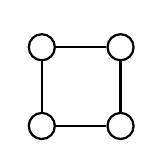
\begin{tikzpicture}[scale=1,
  thick,main node/.style={circle,draw,font=\sffamily\bfseries,minimum size=3mm}]

  \node[main node] (1) at (0,0) {};
  \node[main node] (2) at (0,1){};
  \node[main node] (3) at (1,1){};
  \node[main node] (4) at (1,0) {};

  \path[every node/.style={font=\sffamily\small}]
   (1) edge node[above]{}(2)
   (2) edge node[above]{}(3)
   (3) edge node[above]{}(4)
   (1) edge node[above]{}(4);
\end{tikzpicture}
\hskip10mm
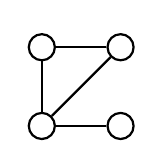
\begin{tikzpicture}[scale=1,
  thick,main node/.style={circle,draw,font=\sffamily\bfseries,minimum size=3mm}]

  \node[main node] (1) at (0,0) {};
  \node[main node] (2) at (0,1){};
  \node[main node] (3) at (1,1){};
  \node[main node] (4) at (1,0) {};

  \path[every node/.style={font=\sffamily\small}]
   (1) edge node[above]{}(2)
   (2) edge node[above]{}(3)
   (3) edge node[above]{}(1)
   (1) edge node[above]{}(4);
\end{tikzpicture}
\hskip10mm
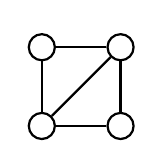
\begin{tikzpicture}[scale=1,
  thick,main node/.style={circle,draw,font=\sffamily\bfseries,minimum size=3mm}]

  \node[main node] (1) at (0,0) {};
  \node[main node] (2) at (0,1){};
  \node[main node] (3) at (1,1){};
  \node[main node] (4) at (1,0) {};

  \path[every node/.style={font=\sffamily\small}]
   (1) edge node[above]{}(2)
   (2) edge node[above]{}(3)
   (3) edge node[above]{}(1)
   (3) edge node[above]{}(4)
   (1) edge node[above]{}(4);
\end{tikzpicture}
\end{center}
\end{comment}

In the latter case, by Corollary~\ref{cor:|x-x|}, there is a geodesic graph $\~\Gamma$ in $\SS^2$ isometric to $\Gamma$;
denote its vertexes by $\~\xi_1,\~\xi_2,\~\xi_3,\~\xi_4\in \SS^2$.
Let $\~p_1$, $\~p_2$, $\~x_1$, $\~x_2$, $\~x_3$, $\~x_4$ be the vertexes of the corresponding pivotal tree in $\HH$;
that is, $\xi_i$ is the normal direction of the half-plane thru $\~x_i$ with $(\~p_1,\~p_2)$ as the boundary line.

Note that in this case
\[\measuredangle(\~\xi_i,\~\xi_j)\ge \alpha_{i,j}\]
for any pair $(i,j)$.
Indeed, if $x_i$ is adjacent to $x_j$ in $\Gamma$ then we have the equality holds;
otherwise the inequality follows from the triangle inequality in $\SS^2$.

\begin{comment}
\begin{wrapfigure}{r}{14 mm}
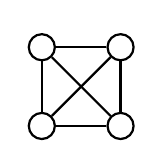
\begin{tikzpicture}[scale=1,
  thick,main node/.style={circle,draw,font=\sffamily\bfseries,minimum size=3mm}]

  \node[main node] (1) at (0,0) {};
  \node[main node] (2) at (0,1){};
  \node[main node] (3) at (1,1){};
  \node[main node] (4) at (1,0) {};

  \path[every node/.style={font=\sffamily\small}]
   (1) edge node[above]{}(2)
   (2) edge node[above]{}(3)
   (2) edge node[above]{}(4)
   (3) edge node[above]{}(1)
   (3) edge node[above]{}(4)
   (1) edge node[above]{}(4);
\end{tikzpicture}
\end{wrapfigure}
\end{comment}

It remains to consider the case when $\Gamma$ is the complete graph (see the diagram). 
Remove the edge $(\xi_3,\xi_4)$ from $\Gamma$;
denote the obtained graph by $\Gamma'$.
Note that there is geodesic graph $\~\Gamma'$ in $\SS^2$ which is isometric to $\Gamma'$;
denote by $\~\xi_1,\~\xi_2,\~\xi_3,\~\xi_4$ the corresponding vertexes in $\~\Gamma'$.
We can (and will) assume that the vertexes $\~\xi_3$ and $\~\xi_4$ lie on the opposite side from the equator containing $[\~\xi_1,\~\xi_2]$.
Let $\~p_1$, $\~p_2$, $\~x_1$, $\~x_2$, $\~x_3$, $\~x_4\in \HH$ be the corresponding pivotal configuration;
that is, $\~\xi_i$ is the normal direction of the half-plane $\~p_1\~p_2\~x_i$ to the line $\~p_1\~p_2$.

Note that by construction, we have 
\[|\~x_i-\~x_j|_\HH\ge|x_i-x_j|_A\]
for each pair $i<j$ except $(3,4)$.


Denote by $\~K$ the convex hull of $\~x_1,\~x_2,\~x_3,\~x_4$ in $\HH$
and by $\~K'$ the convex hull of $\~\xi_1,\~\xi_2,\~\xi_3,\~\xi_4$ in $\SS^2$.


Assume the interior of $\~K$ intersects the line $\~p_1\~p_2$;
or equivalently $\~K'=\SS^2$.
Then by the rigidity lemma, we have 
\[|\~x_3-\~x_4|_\HH\ge|x_3-x_4|_A.\]
In particular, the array $\~p_1$, $\~p_2$, $\~x_1$, $\~x_2$, $\~x_3$, $\~x_4\in \HH$ satisfies the tree comparison.

\begin{wrapfigure}{r}{25 mm}
\begin{lpic}[t(-0 mm),b(-0 mm),r(0 mm),l(0 mm)]{pics/K-shtrikh(1)}
\lbl[r]{1,22;$\xi_1$}
\lbl[tl]{13,22;$\xi_2$}
\lbl[rt]{1.5,1;$\xi_3$}
\lbl[b]{22,34;$\xi_4$}
\lbl[l]{4,44;$\xi_4'$}
\lbl{6,17;{\color{white}$\~K'$}}
\end{lpic}
\end{wrapfigure}

In the remaining case $\~K'\ne \SS^2$, the boundary $\partial_{\SS^2}\~K'$ is nonempty; moreover it contains at least 3 of the vertexes $\~\xi_1,\~\xi_2,\~\xi_3,\~\xi_4$.
Without loss of generality we may assume that $\~\xi_1\in \partial_{\SS^2}K$.
Denote by $\~\xi_4'$ the point on the extension of $[\~\xi_3,\~\xi_1]$ behind $\~\xi_1$ such that $|\~\xi_1-\~\xi_4'|_{\SS^2}=|\~\xi_1-\~\xi_4|_{\SS^2}$.
Since the increasing of angle increase the opposite side, we have
\begin{align*}
|\~\xi_2-\~\xi_4'|_{\SS^2}&\ge|\~\xi_2-\~\xi_4|_{\SS^2}=
\\
&=\alpha_{2,4}.
\end{align*}
Note that 
\[
|\~\xi_3-\~\xi_4'|_{\SS^2}=\min\{\,\alpha_{1,3}+\alpha_{1,4},\,\pi-(\alpha_{1,3}+\alpha_{1,4})\,\} 
\]
Since $\Gamma$ is complete, we have 
\[\alpha_{1,3}+\alpha_{1,4}\ge \alpha_{3,4}\]
and by Corollary~\ref{cor:|x-x|},
\[\alpha_{1,3}+\alpha_{1,4}+\alpha_{3,4}\le 2\cdot\pi.\]
Therefore 
\[
|\~\xi_3-\~\xi_4'|_{\SS^2}\ge \alpha_{3,4}.
\]
It follows that the pivotal configuration with normal directions $\~\xi_1,\~\xi_2,\~\xi_3,\~\xi_4'$ satisfies the definition of tree comparison.
\qeds



